\chapter{}

\paragraph\ 
%The appendices play an important role in the record-keeping of the valuable data gathered for and during the project. The appendices may contain different types of data, e.g., questionnaire and survey forms, raw experimental data, raw analytical data, drawings, computer program listings, and detailed derivations of certain expressions used in the main body of the report.

The appendix contains a list of acronyms used in the report, screenshots, and supporting information relevant to the work in the main body of the report.

\vspace{1cm}

\section*{List of Acronyms}
\begin{acronym}
 %chap1
  \acro{ZB}{Zettabyte}
  \acro{IG}{Information Governance}
  \acro{GDPR}{General Data Protection Regulation}
  \acro{DPD}{Data Protection Directive}
  \acro{EU}{European Union}
  \acro{ML}{Machine Learning}
  \acro{AI}{Artificial Intelligence}
  \acro{IR}{Information Retrieval}
  \acro{IBM}{International Business Machines}
  \acro{EIM}{Enterprise Information Management}
  \acro{PII}{Personal Identifiable Information}
 %chap2 
  \acro{NLU}{Natural Language Understanding}
  \acro{NER}{Named Entity Recognition}
  \acro{IPVS}{Institute for Parallel and Distributed Systems}
  \acro{API}{Application Programming Interface}
  \acro{REST}{Representational State Transfer Application}
  \acro{SDK}{Software Development Kit}
  \acro{NLP}{Natural Language Processing}
  \acro{AWS}{Amazon Web Services}
  \acro{OCR}{Optical Character Recognition}
  \acro{pdf}{Portable Document Format}
  \acro{jpeg}{Joint Photographic Experts Group}
  \acro{png}{Portable Network Graphics}
  \acro{UCI}{University of California Irvine}
  %chap3 
  \acro{IPVS}{Institute for Parallel and Distributed Systems}
  \acro{DCA}{Development Credit Authority}
  \acro{USAID}{United States Agency for International Development}
  %chap4
  \acro{CLI}{Command Line Interface}
  \acro{UI}{User Interface}
  %chap5
  \acro{ISO}{International Organization for Standardization}
  \acro{SCC}{Standard Contractual Clauses}
  \acro{EEA}{European Economic Area}
  \acro{FAQ}{Frequently Asked Questions}
  \acro{MFA}{multi-factor authentication}
  \acro{SSL}{Secure Sockets Layer}
  \acro{TLS}{Transport Layer Security}
  \acro{IEC}{International Electrotechnical Commission}
  \acro{url}{Uniform Resource Locator}
\end{acronym}
%\printacronyms

\newpage

\section*{Snippets and screenshots}
\underline{From Chapter 3: Dataset: Dataset 3:}
\paragraph\ Zoomed-in snippet of Dataset 3 taken in two halves as the dataset had many columns (A-R) to fit in a single image.
\begin {figure}[ht]
\centering
\adjustbox{frame}{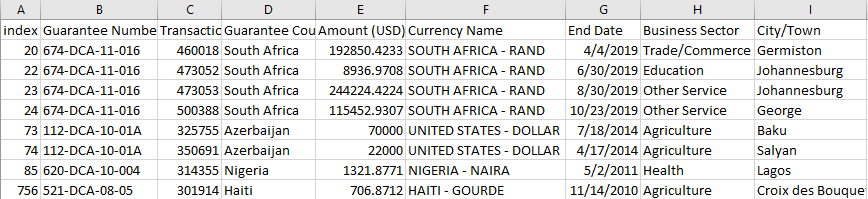
\includegraphics[scale=0.747]{images/Appendix_images/dca_dataset1.png}}
\caption{Dataset 3: \acs{DCA} Loan Dataset Part-1 (First half of data columns A-I)}
\label{dcaloandataset1}
\end {figure}

\begin {figure}[ht]
\centering
\adjustbox{frame}{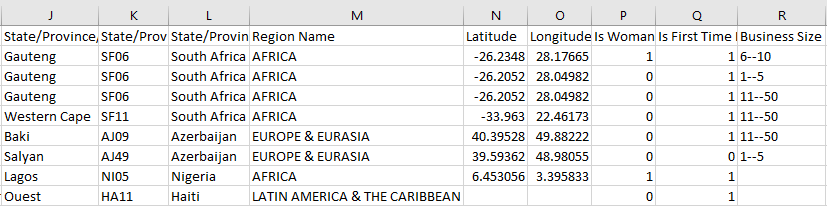
\includegraphics[scale=0.78]{images/Appendix_images/dca_dataset2.png}}
\caption{Dataset 3: \acs{DCA} Loan Dataset Part-2 (Second half of data columns J-R)}
\label{dcaloandataset2}
\end {figure}

\newpage

\underline{From Chapter 4: The test plan:}
\paragraph\ 
The snippet of an example from the sample dataset showing the (full) document view \ref{sampledatadetail} and the concise version of it \ref{sampledataconcise}.

\begin {figure}[h]
    \centering
    \adjustbox{frame}{
\includegraphics[height=17cm, width=1\textwidth]{images/Appendix_images/sample_dataset_detailed.png}}
    \caption{1st page of the full example document from sample dataset}
    \label{sampledatadetail}
\end {figure}

\vspace{5cm}

\begin {figure}[h]
    \centering
    \adjustbox{frame}{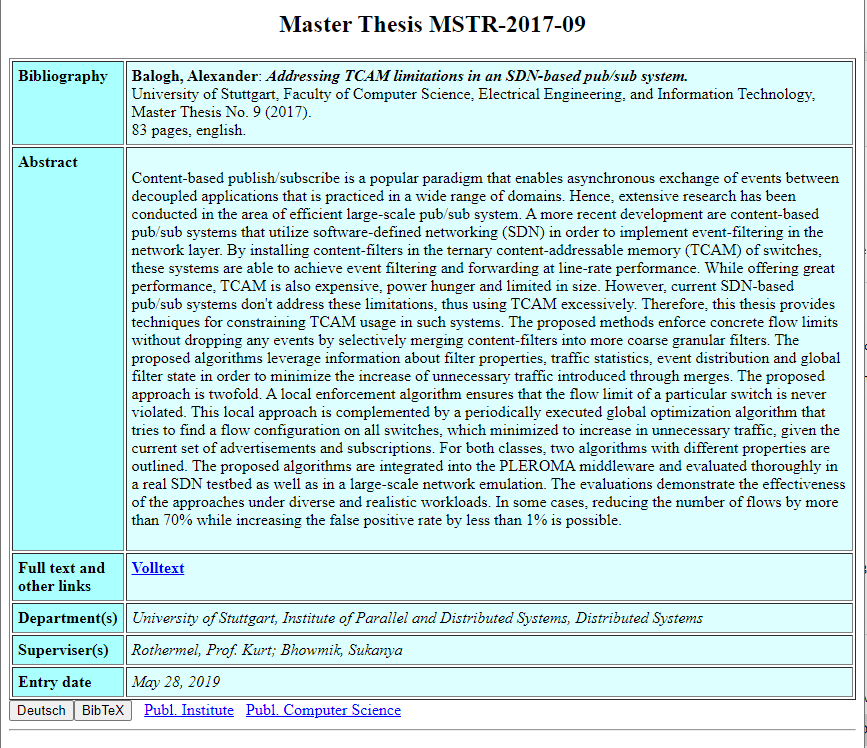
\includegraphics[height=15cm, width=1\textwidth]{images/Appendix_images/sample_dataset.png}}
    \caption{Overview about the example document from sample dataset}
    \label{sampledataconcise}
\end {figure}

%\vspace{1.5cm}
%\vspace{6cm}

\newpage

\underline{From Chapter 4: Implementation:}
\begin{enumerate}
    \item A snapshot of Azure resources created in the portal during this testing:
        \begin {figure}[ht]
            \centering
            \adjustbox{frame}{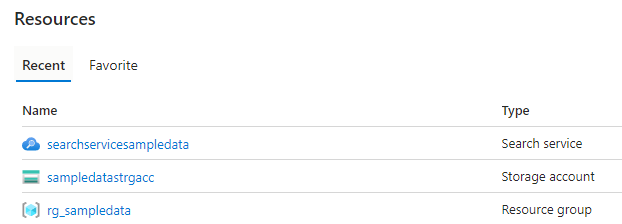
\includegraphics[scale=0.9]{images/Appendix_images/azure_resources_created.png}}
            \caption{Azure resources created with names and resource types}
            \label{azureresources}
        \end {figure}
    \item A snippet of available Cognitive skillsets to choose from:
        \begin {figure}[h!h]
            \centering
            \adjustbox{frame}{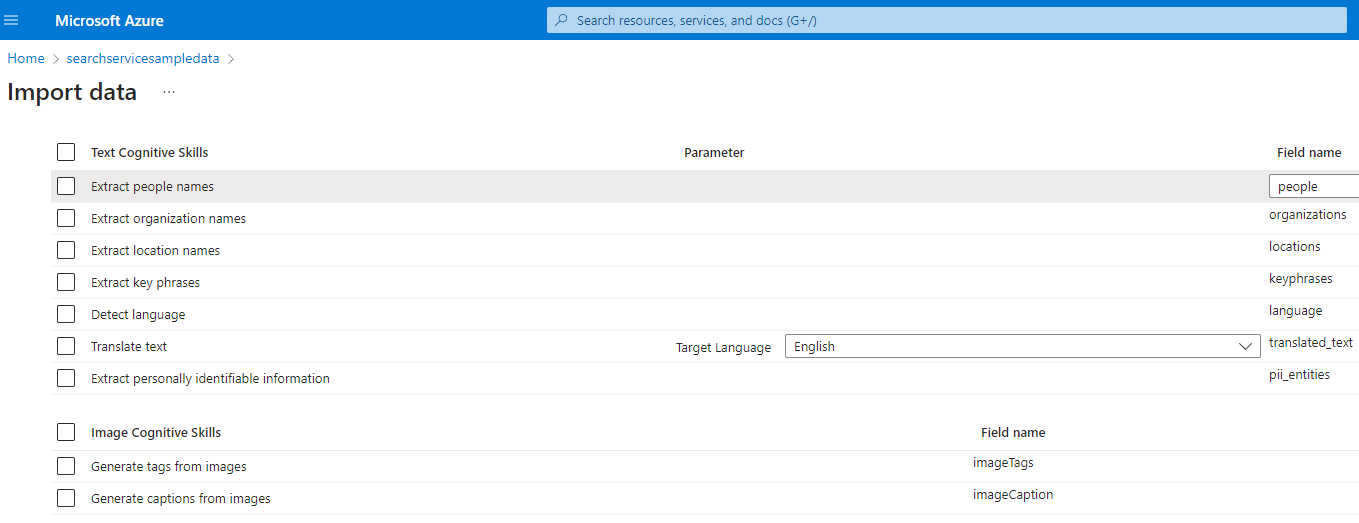
\includegraphics[width=1\textwidth, height=8cm]{images/Appendix_images/cog_skillset.png}}
            \caption{Cognitive skillset list}
            \label{cogskillset}
        \end {figure}
    \newpage
    \item A snippet showing language options to choose for targeted language translation:
        \begin {figure}[h!h]
            \centering
            \adjustbox{frame}{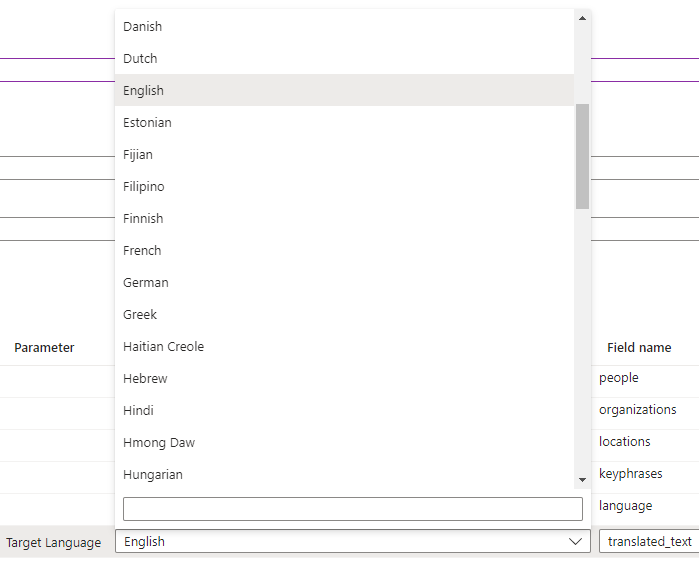
\includegraphics[scale=0.62]{images/Appendix_images/translate_lang_64.png}}
            \caption{Language options for translation}
            \label{translang}
        \end {figure}
    \item A snippet showing PII tryout with one of the sample texts used for testing:
        \begin {figure}[h!h]
            \centering
            \adjustbox{frame}{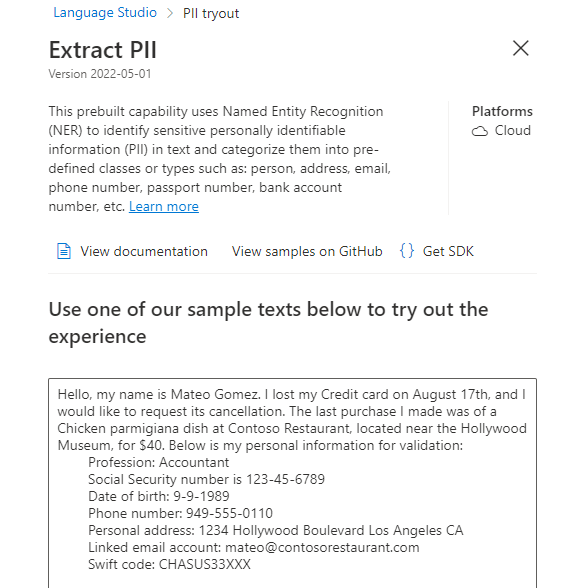
\includegraphics[scale=0.62]{images/Appendix_images/pii_tryout1.png}}
            \caption{Snippet of sample banking text used as input for PII tryout}
            \label{piitryout}
        \end {figure}
    \newpage
    \item A snippet showing sample texts options provided and the selected text for PII tryout:
    \begin {figure}[h!h]
        \centering
        \adjustbox{frame}{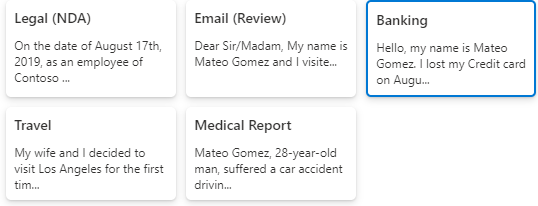
\includegraphics[scale=0.72]{images/Appendix_images/sample_texts.png}}
        \caption{Sample texts options for the user to try PII extraction}
        \label{sampletexts}
    \end {figure}
    \item A snippet showing \acs{PII} entities found in the text. Each PII has confidence mentioned along with the entity type. \textit{Subtype} is also mentioned for applicable fields ('Date' for 'DateTime'). We can also see that there is a significant difference in the confidence levels of the \textit{Person} PII identified; the one with the full name of the person has rightly been denoted with higher confidence than the (only first) name mentioned in the email address.
        \begin {figure}[h!h]
            \centering
            \adjustbox{frame}{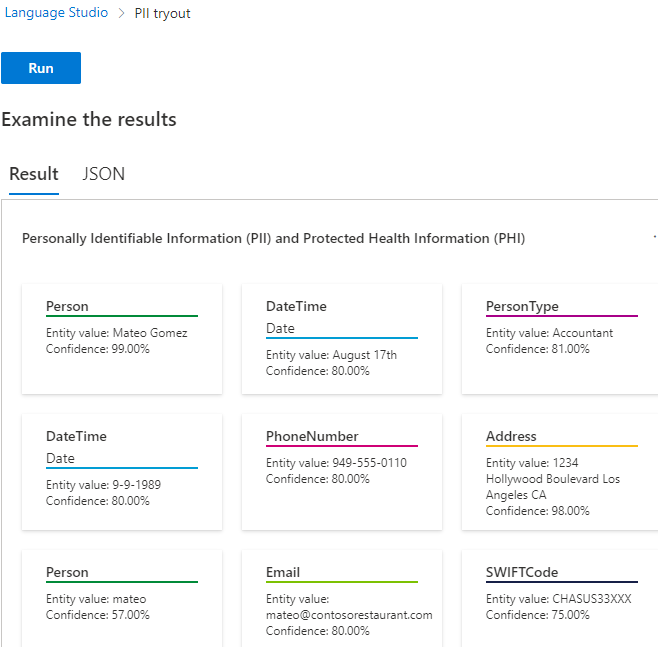
\includegraphics[scale=0.7]{images/Appendix_images/pii_results.png}}
            \caption{Snippet showing the results of PII extraction on sample banking text}
            \label{piires}
        \end {figure}
    \newpage
    \item A snippet of the original text with the identified PIIs highlighted:
        \begin {figure}[h!h]
            \centering
            \adjustbox{frame}{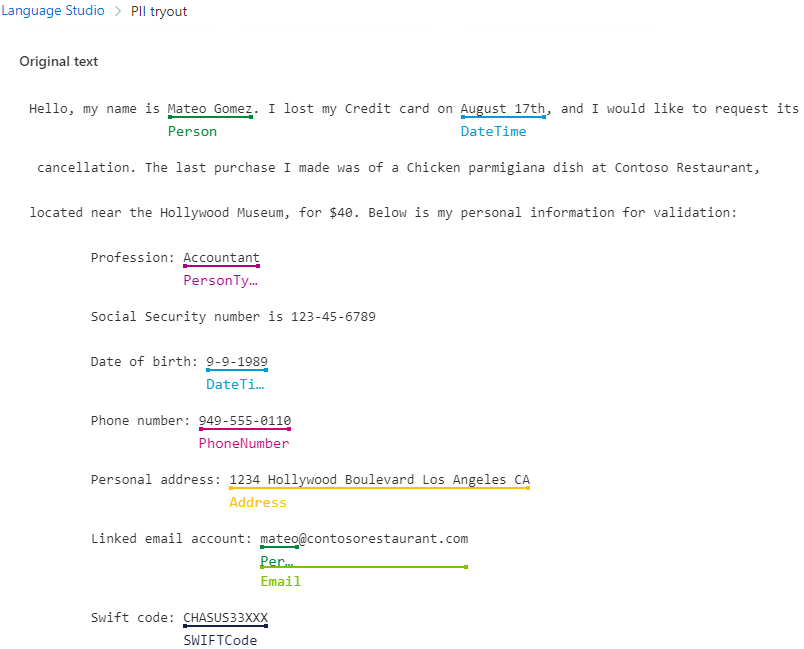
\includegraphics[scale=0.65]{images/Appendix_images/pii_og_text.png}}
            \caption{PII tryout results on the original text}
            \label{piiogtext}
        \end {figure}
    \item A snippet showing NER results with the same banking texts used for the PII tryout:
        \begin {figure}[h!h]
            \centering
            \adjustbox{frame}{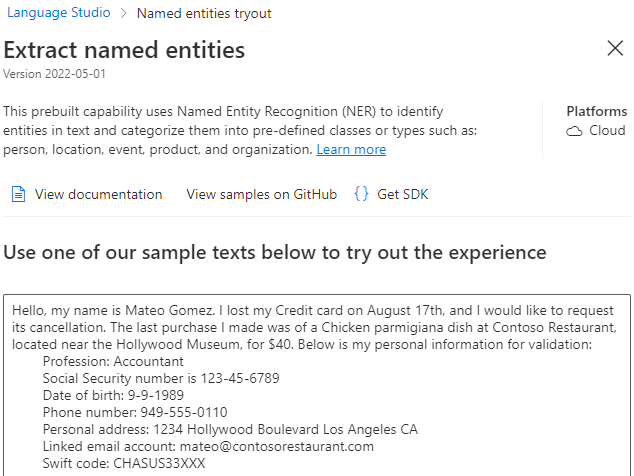
\includegraphics[scale=0.6]{images/Appendix_images/ner_tryout1.png}}
            \caption{Snippet of sample banking text used as input for \acs{NER} tryout}
            \label{nertryout}
        \end {figure}
    \clearpage
    \newpage
    \item A snippet showing the named entities found in the text. Each entity has the confidence mentioned along with the entity category. \textit{Subtype} is also mentioned for applicable fields ('Currency' and 'Number' for 'Quantity').
        \begin {figure}[h!h]
            \centering
            \adjustbox{frame}{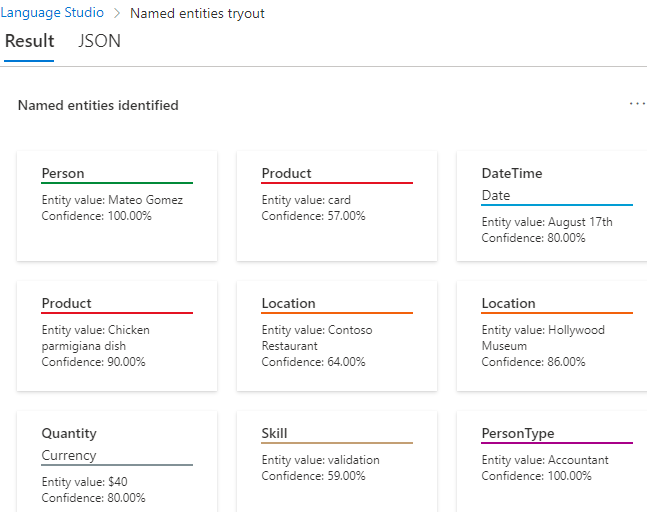
\includegraphics[scale=0.62]{images/Appendix_images/ner_results1.png}}
            \caption{Snippet showing part-1 of the results of NER extraction on sample banking text}
            \label{nerres1}
        \end {figure}
    \item A snippet showing the continued cards of named entities found in the text. 
    \begin {figure}[h!h]
        \centering
        \adjustbox{frame}{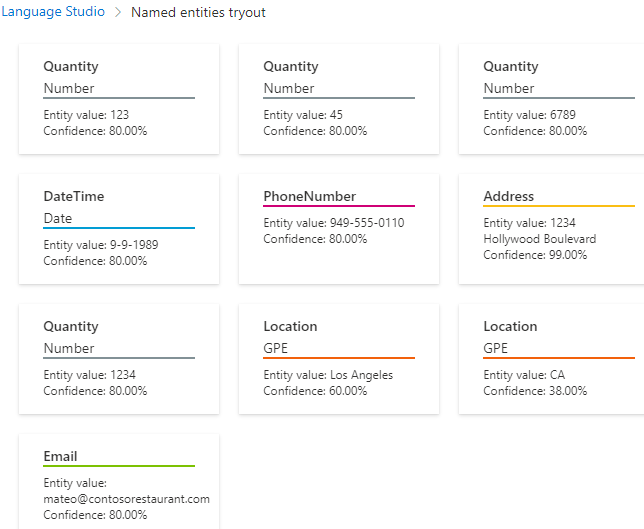
\includegraphics[scale=0.65]{images/Appendix_images/ner_results2.png}}
        \caption{Snippet showing part-2 of the results of NER extraction on sample banking text}
        \label{nerres2}
    \end {figure}
    \newpage
    \item A snippet showing the option provided for users to view the extracted entities by:\\
    1) sorting them based on categories or order of occurrence or confidence levels and \\
    2) filtering them based on the categories.
        \begin {figure}[h!h]
            \centering
            \adjustbox{frame}{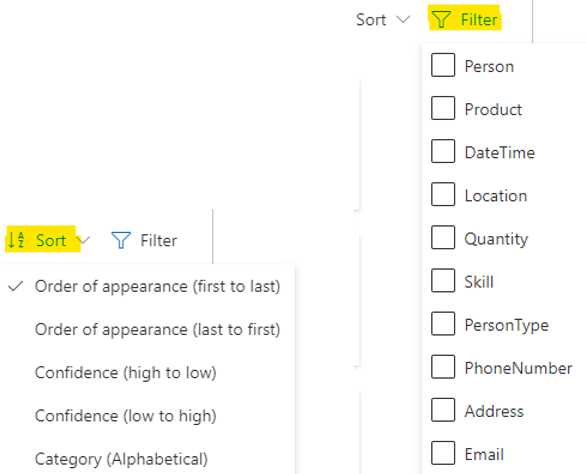
\includegraphics[scale=0.5]{images/Appendix_images/ner_res_filter_sort.png}}
            \caption{Snippet showing sorting and filtering options to view the results}
            \label{sortfilternerres}
        \end {figure}
    \item A snippet of the original text with the identified named entities highlighted:
        \begin {figure}[h!h]
            \centering
            \adjustbox{frame}{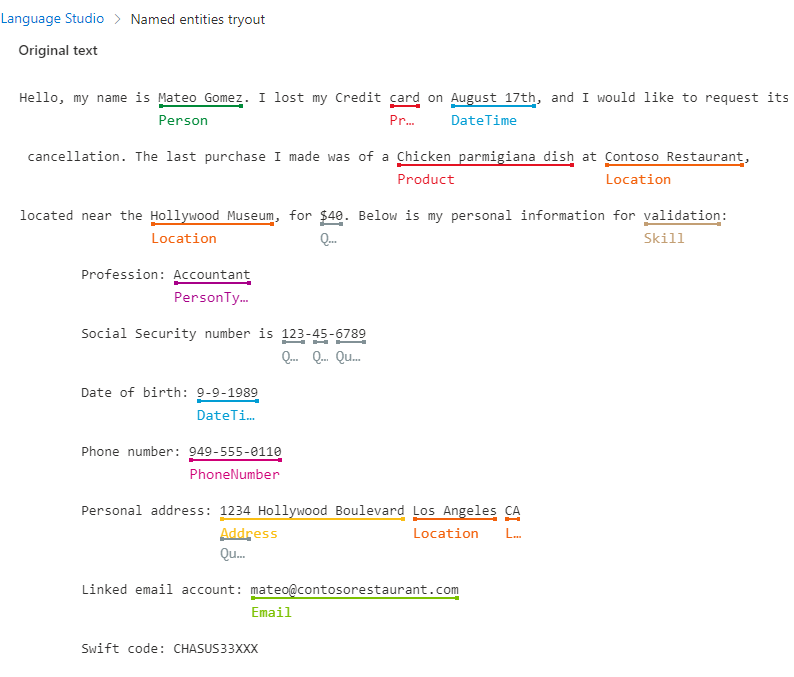
\includegraphics[scale=0.639]{images/Appendix_images/ner_og_text.png}}
            \caption{\acs{NER} tryout results on the original text}
            \label{nerogtext}
        \end {figure}
    \item A snippet of choice to enable the opinion mining in Sentiment Analysis tryout:
        \begin {figure}[h!h]
            \centering
            \adjustbox{frame}{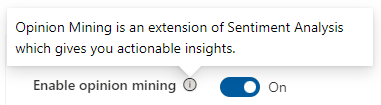
\includegraphics[scale=0.7]{images/Appendix_images/sa_enable_opinion1.png}}
            \caption{Enabling opinion mining}
            \label{enableopinion}
        \end {figure}
    \item A snippet of the original text after performing sentiment analysis and opinion mining:
        \begin {figure}[h!h]
            \centering
            \adjustbox{frame}{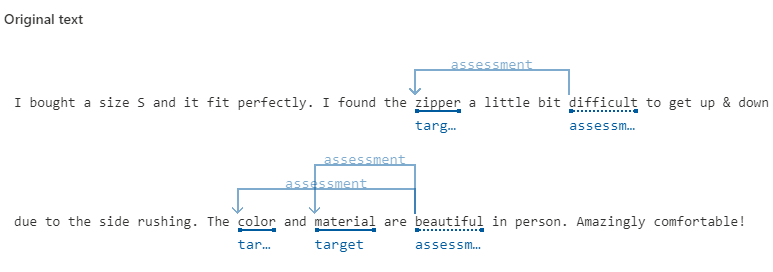
\includegraphics[scale=0.7]{images/Appendix_images/sa_opinion_res.png}}
            \caption{Snippet of the result after enabling opinion mining}
            \label{opinionres}
        \end {figure}
    \item A snippet of the results for sentence-2 in specific after enabling opinion miming:
        \begin {figure}[h!h]
            \centering
            \adjustbox{frame}{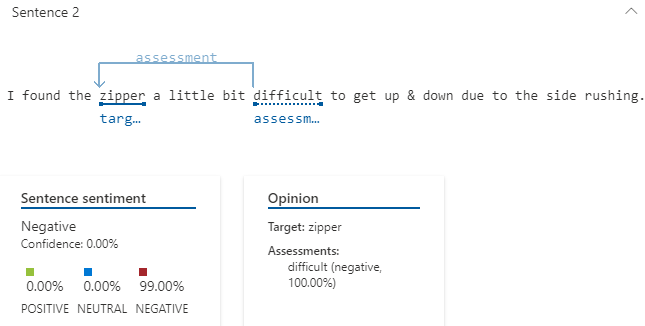
\includegraphics[scale=0.8]{images/Appendix_images/sa_opinion_res1.png}}
            \caption{Snippet of result for sentence-2 after enabling opinion mining}
            \label{opinionres}
        \end {figure}
    \item A snippet of the results for sentence-1 and sentence-2 to note the difference in confidence levels of sentiment analysis even though the sentence is classified with more than 90\% of a particular sentiment:
        \begin {figure}[h!h]
            \centering
            \adjustbox{frame}{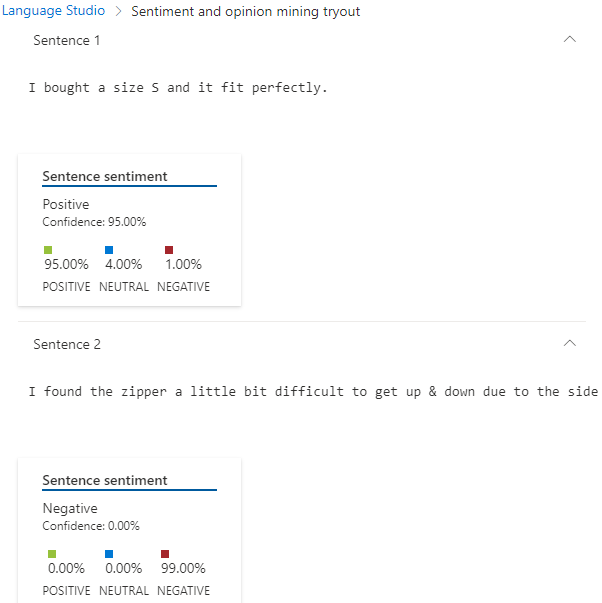
\includegraphics[scale=0.62]{images/Appendix_images/sa_confidence_levels.png}}
            \caption{Result for sentence-1 and sentence-2 to note the difference in confidence levels}
            \label{saconfilevel}
        \end {figure}
        \begin {figure}[h!h]
            \centering
            \adjustbox{frame}{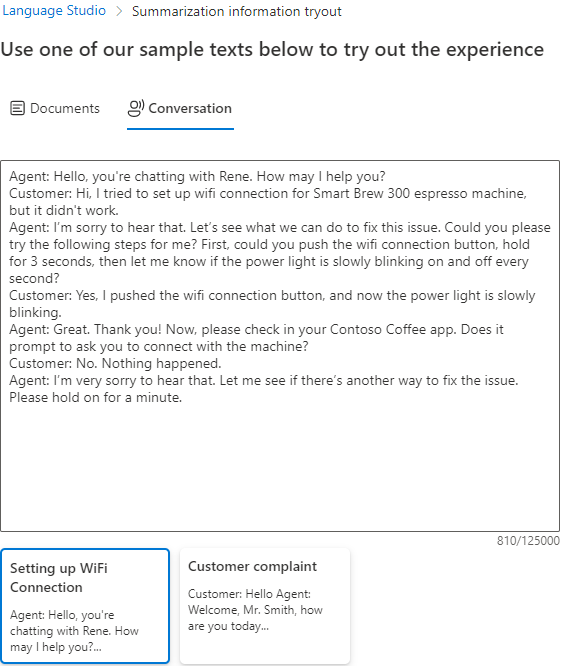
\includegraphics[scale=0.65]{images/Appendix_images/summ_tryout.png}}
            \caption{Snippet of input conversation for summarization}
            \label{summinput}
        \end {figure}
    \clearpage
    \newpage
    \item A snippet of the conversation is given as input for summarization. There were two options available, used the WiFi connection sample as seen in Figure \ref{summinput}.
        
    \item \label{item:tcfeature} For custom text classification, as there were no sample texts available, the author tried to create a project for it using the already created language resource \textit{coglangservice} \ref{langres}. But it was not shown in the portal when the author tried to add it to the project as seen in Figure \ref{textclass1}. The author even tried creating a new resource from the link provided at the bottom of the pop-up. The resource would get created successfully but still not appear in the list of resources. In Figure \ref{textclass2} requirements are clear that a language resource should be added but the language resource \textit{coglangservice} created was not recognized or shown in the list. It could be possible that this was due to the fact that this resource was created using the free tier pricing method available in student subscription:
        \begin {figure}[h!h]
            \centering
            \adjustbox{frame}{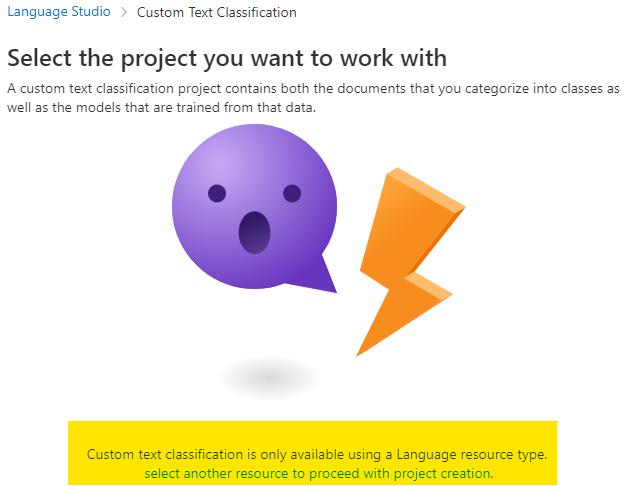
\includegraphics[scale=0.95]{images/Appendix_images/text_classification_error.png}}
            \caption{Snippet showing a requirement for using custom text classification}
            \label{textclass2}
        \end {figure}
        \begin {figure}[h!h]
            \centering
            \adjustbox{frame}{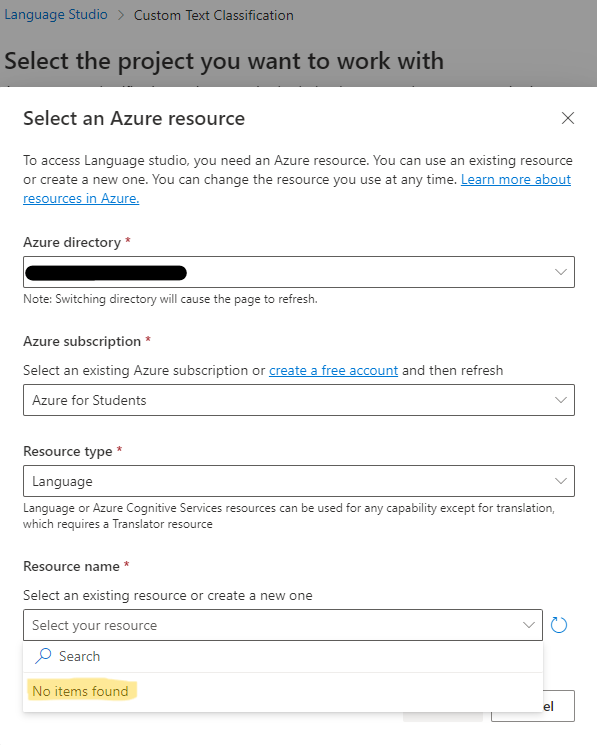
\includegraphics[scale=0.82]{images/Appendix_images/text_classification.png}}
            \caption{Snippet showing that the created language resource \textit{coglangservice} is not shown in list of resources}
            \label{textclass1}
        \end {figure}
        %\vspace{2cm} 
    \newpage
    \item \label{item:neutral} During testing, it was seen that IBM did not identify neutral much, so tested both service providers with a neutral statement \textit{'The price tags on cosmetic products were changed'}. The statement could either be positive or negative and has no clear sentiment; the expectation would be to classify it into a Neutral class. The results of Azure's analysis can be seen in Figure \ref{azsaneut} and that of IBM can be seen in Figure \ref{ibmsaneut}.
        \begin {figure}[h!h]
            \centering
            \adjustbox{frame}{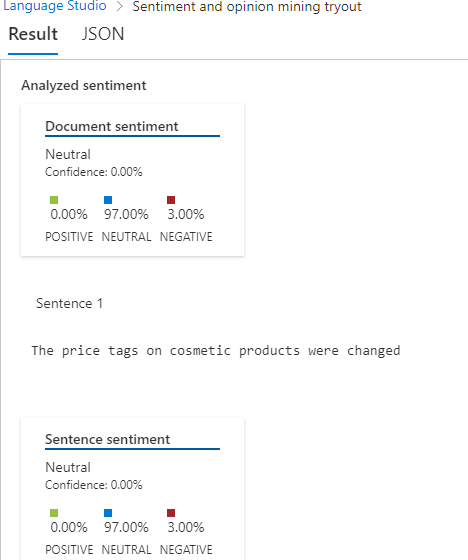
\includegraphics[scale=0.77]{images/Appendix_images/azure_sa_neutral.png}}
            \caption{Snippet showing the sentiment analysis results of Azure for the neutral input}
            \label{azsaneut}
        \end {figure}
        \begin {figure}[h!h]
            \centering
            \adjustbox{frame}{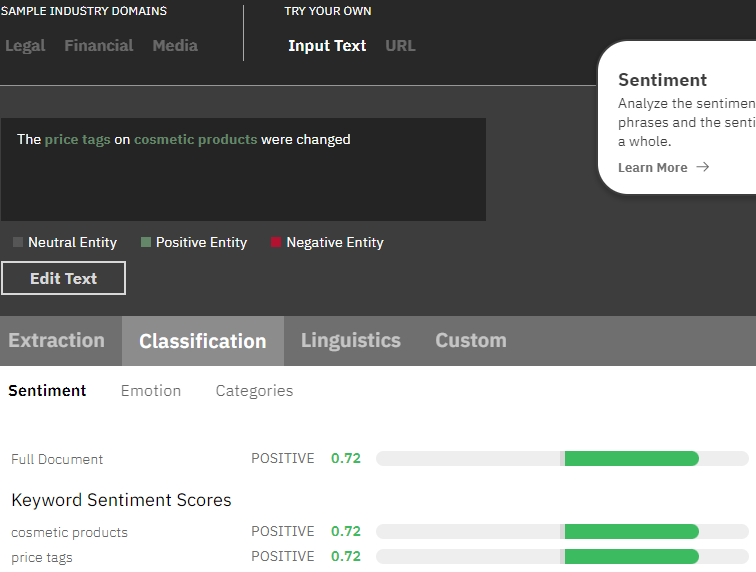
\includegraphics[scale=0.65]{images/Appendix_images/ibm_sa_neutral.png}}
            \caption{Snippet showing the sentiment analysis results of IBM for the neutral input}
            \label{ibmsaneut}
        \end {figure}
    \clearpage 
\end{enumerate}

\clearpage
\newpage
\underline{Support Responses for access:}
\paragraph\ 
The snippets of email responses from support teams of Microsoft Azure and AWS can be found in the Figures below. Response from Microsoft Azure is in \ref{azuresupportresp} where they mentioned that Azure for students is the only option to use but it exhausts in 1 month. After which, the only other method is to purchase a subscription. The response from AWS is split in \ref{awssupportresp1} and \ref{awssupportresp2} as it was a bit long to be covered in one screenshot.

\begin {figure}[ht]
    \centering
    \adjustbox{frame}{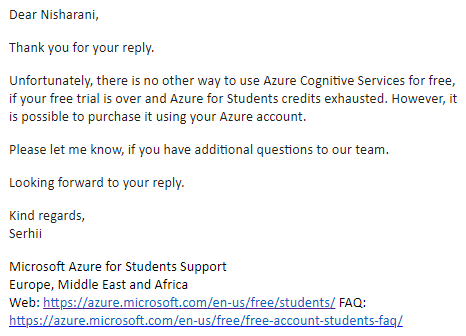
\includegraphics[scale=1]{images/Appendix_images/MS_support.png}}
    \caption{Support response from Microsoft Azure team}
    \label{azuresupportresp}
\end {figure}

\begin {figure}[ht]
    \centering
    \adjustbox{frame}{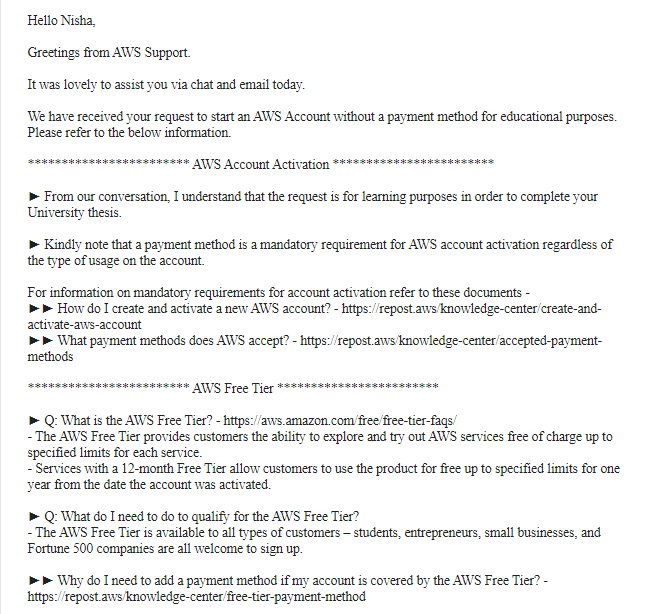
\includegraphics[height=12cm, width=0.9\textwidth]{images/Appendix_images/AWS_support1.png}}
    \caption{Support response from Amazon Web Services team part-1}
    \label{awssupportresp1}
\end {figure}

\begin{figure}[h!h]
  \centering
  \adjustbox{frame}{\includegraphics[height=9cm, width=0.9\textwidth]{images/Appendix_images/AWS\_support2.png}}
  \caption{Support response from Amazon Web Services team part-2}
  \label{awssupportresp2}
\end{figure}
\clearpage
%\vspace{1.5cm}

\newpage
\underline{From Chapter 5: \acs{IR} features test results:}
\paragraph\ Snippets to provide more details and information about the testing and results on 3 datasets are shown in this section.
\begin{itemize}
    \item Input is possible in the form of characters or input files. But the input is limited to 5000 characters and the input file type is limited to type 'txt' file as seen in Figure \ref{azinputlimitation}. If a file with more characters is uploaded, the algorithm trims it and processes only the first 5000 characters. But when browsed and uploaded a 'csv' file, it accepted and trimmed the content to the first 5000 characters. This limitation was for both free-tier resources and standard resources.
    \begin{figure}[h!h]
      \centering
      \adjustbox{frame}{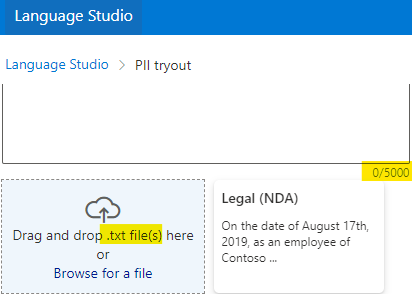
\includegraphics[scale=0.85]{images/Appendix_images/character_limit_file_type.png}}
      \caption{Snippet showing the input limitations in Azure testing}
      \label{azinputlimitation}
    \end{figure}
    \item Snippet of the converted 'txt' file which was input for testing the \acs{PII} feature is seen in Figure \ref{aztextinputfile}. 
    \begin{figure}[h!h]
      \centering
      \adjustbox{frame}{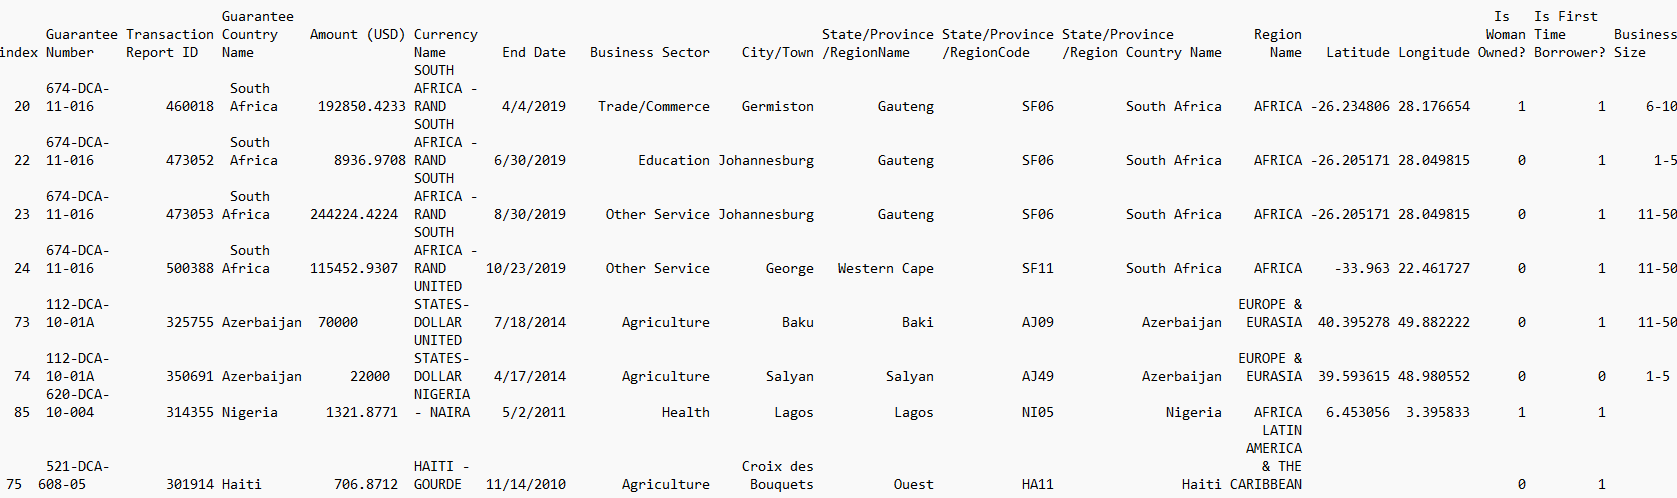
\includegraphics[width=1\textwidth]{images/Appendix_images/converted_text_file.png}}
      \caption{Snippet of converted 'txt' file used for Azure testing}
      \label{aztextinputfile}
    \end{figure}
    \item Snippet of uploading the 25,119 image files from Dataset-1 into the Azure Blob Storage container. Used the same Azure storage service but added a new container \textit{ocrd1} for this dataset and uploaded the files. It took a while to upload the files. A snippet is shown in Figure \ref{ocrd1upload}. Though the upload was successful. When querying, we saw that there were only 36 documents that were loaded and being queried. 
    \begin{figure}[h!h]
      \centering
      \adjustbox{frame}{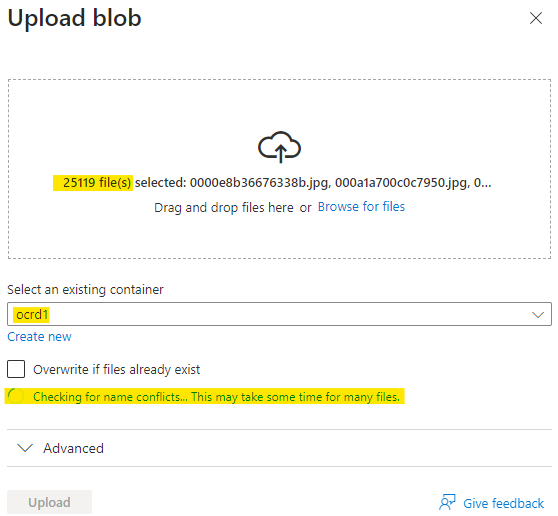
\includegraphics[scale=1]{images/Appendix_images/ocr_upload_d1.png}}
      \caption{Snippet of uploading dataset-1 to Azure storage for testing}
      \label{ocrd1upload}
    \end{figure}
    \newpage
    \item Snippet of results of the query \texttt{’search=*\&\$count=true’} on dataset-2 index are shown in Figure \ref{sentiocrres}. It shows all the fields and information extracted from one image.
    \begin{figure}[h!h]
      \centering
      \adjustbox{frame}{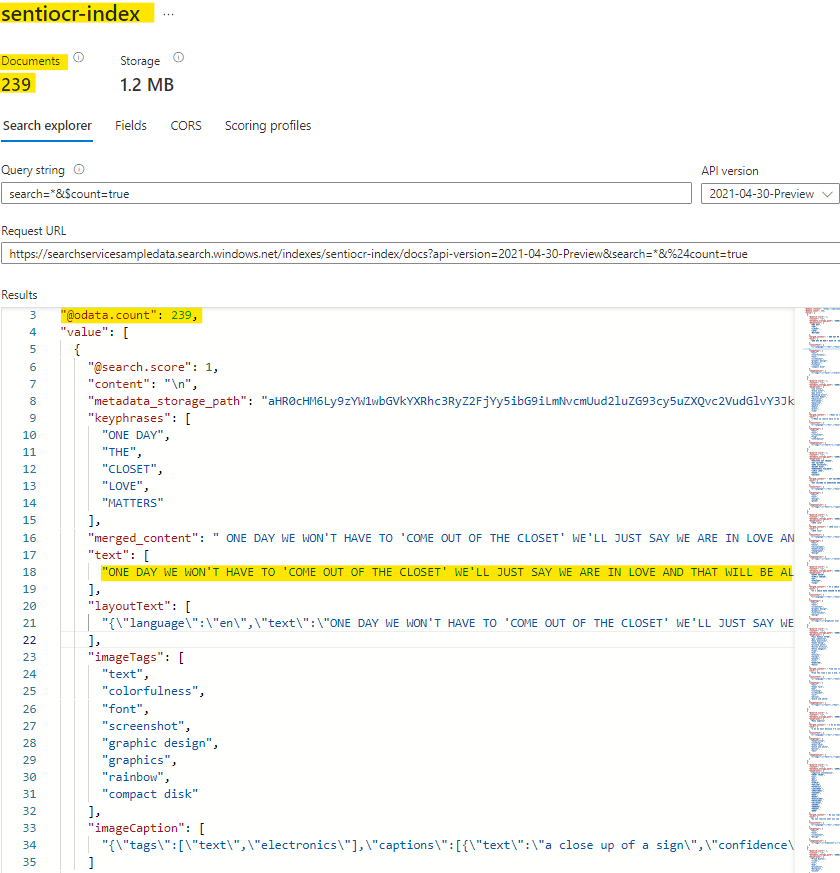
\includegraphics[scale=0.745]{images/Appendix_images/senti_ocr_output1_d2.png}}
      \caption{Full list of fields shown for one image in \acs{OCR}}
      \label{sentiocrres}
    \end{figure}
    %\newpage
    \item \label{item:textocrresults} Snippet of results of the query \texttt{’search=*\&\$count=true’} on dataset-1 index are shown in Figure \ref{textocrres1}. It shows all the fields and information extracted from one image.
    \begin{figure}[h!h]
      \centering
      \adjustbox{frame}{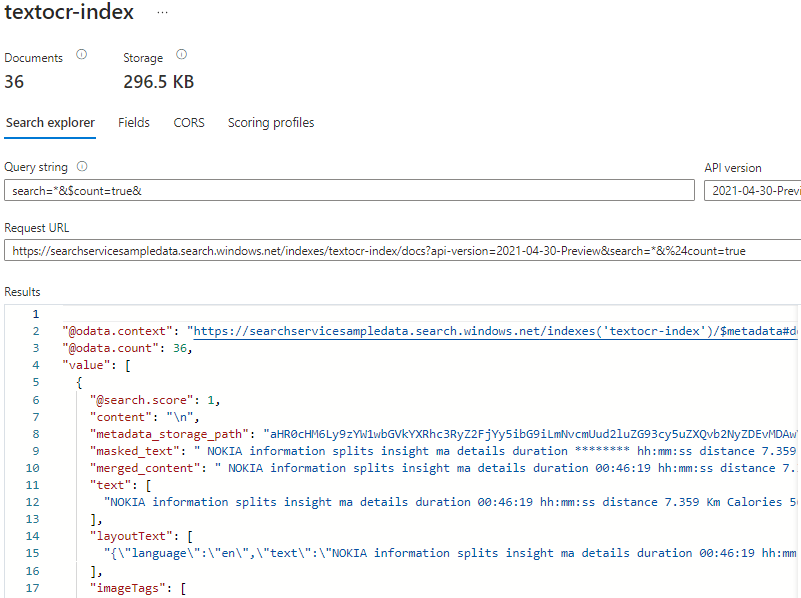
\includegraphics[scale=0.687]{images/Appendix_images/text_ocr_output1_d1.png}}
      \caption{Full list of fields shown for one image in \acs{OCR} part-1}
      \label{textocrres1}
    \end{figure}
    \begin{figure}[h!h]
      \centering
      \adjustbox{frame}{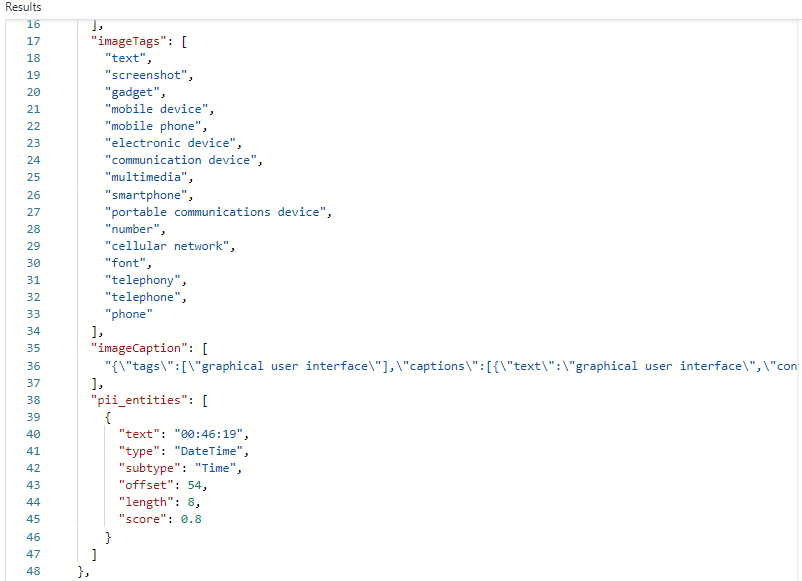
\includegraphics[scale=0.687]{images/Appendix_images/text_ocr_output2_d1.png}}
      \caption{Full list of fields shown for one image in \acs{OCR} part-2}
      \label{textocrres2}
    \end{figure}
\end{itemize}

\clearpage
\newpage
\underline{From Chapter 5: \acs{GDPR} readiness: \acs{GDPR} readiness in Google Cloud:}
\paragraph\ 
We can see in Figure \ref{gcworkaccs} that while creating a Google Workspace account (it was mandatory to have one in order to be able to view or download the compliance reports and certificates for Google) it was compulsory to either have a domain or purchase one. Figure \ref{gcworkaccdomains} shows that none of the options were free and hence the author was unable to create a Google Workspace account and was therefore unable to view any compliance certificates of Google.
\begin {figure}[ht]
    \centering
    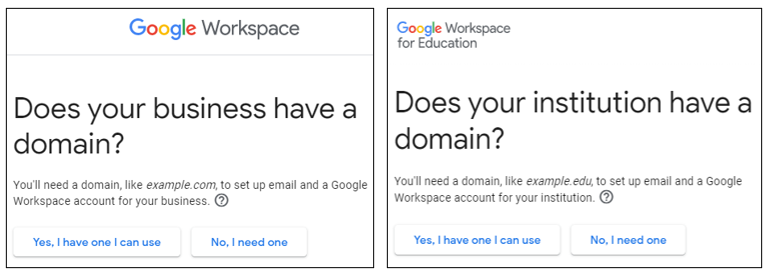
\includegraphics[scale=0.65]{images/Appendix_images/google_workspace.png}
    \caption{Domain options while creating the Google Workspace account for business (left side) and for education (right side)}
    \label{gcworkaccs}
\end {figure}
\begin{comment}
\begin {figure}[ht]
    \centering
    \adjustbox{frame}{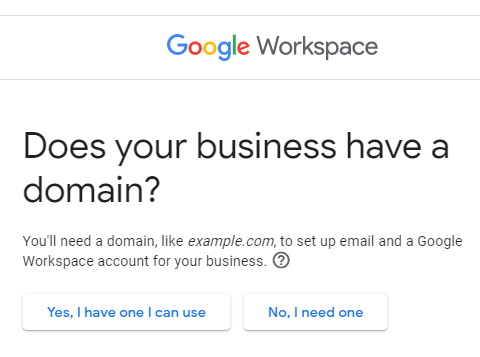
\includegraphics[scale=0.8]{images/Appendix_images/google_workspace1.png}}
    \caption{Creating the Google Workspace account business edition}
    \label{gcworkaccbized}
\end {figure}

\begin {figure}[ht]
    \centering
    \adjustbox{frame}{
\includegraphics[scale=0.8]{images/Appendix_images/google_workspace2.png}}
    \caption{Creating the Google Workspace account for schools}
    \label{gcworkaccschooled}
\end {figure}
\end{comment}
\begin {figure}[h!h]
    \centering
    \adjustbox{frame}{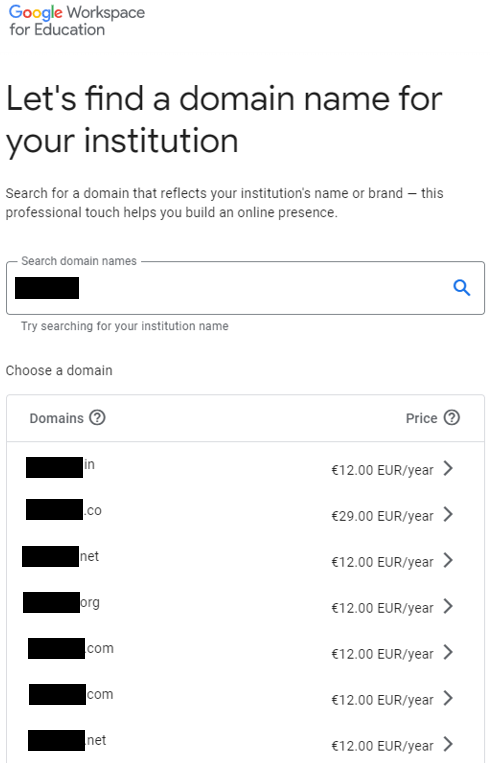
\includegraphics[scale=0.53]{images/Appendix_images/google_workspaceE.png}}
    \caption{Costs for purchasing domains}
    \label{gcworkaccdomains}
\end {figure}